% A lattice L in C with a unit-square fundamental domain, projecting to the
% torus C/L (the same square with opposite edges identified).
% Source: book/tex/riemann-surface/complex-structure.tex (§ The torus C/L).
\documentclass[border=2mm]{standalone}
\usepackage{tikz}
\usepackage{amssymb}
\begin{document}
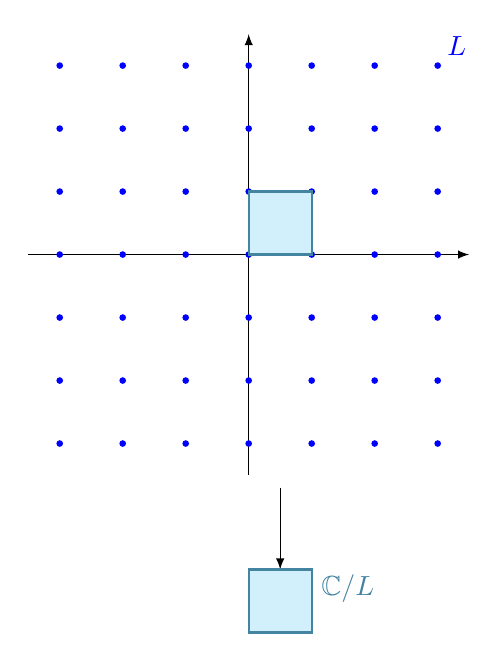
\begin{tikzpicture}[scale=0.8,>=latex]
  \draw[->] (-3.5,0)--(3.5,0); \draw[->] (0,-3.5)--(0,3.5);
  \foreach \x in {-3,...,3}\foreach \y in {-3,...,3}\fill[blue] (\x,\y) circle(1.5pt);
  \filldraw[fill=cyan!18, draw=cyan!60!black, thick] (0,0) rectangle (1,1);
  \node[blue,above right] at (3,3) {$L$};
  \draw[->] (0.5,-3.7)--(0.5,-5.0);
  \filldraw[fill=cyan!18, draw=cyan!60!black, thick] (0,-6) rectangle (1,-5);
  \node[cyan!60!black,right] at (1,-5.3) {$\mathbb{C}/L$};
\end{tikzpicture}
\end{document}
